\chapter{Computer Vision}\label{ch:img_proc}
The computer vision part is the image processing part of the project. Here the machine differentiates the different \lego bricks and their individual colours. Furthermore their pixel position is found to be converted to world coordinates later in the program.
This is done to let the robot use the knowledge of the different colours to automatically assemble the figures with the right coloured bricks.
To find the bricks in the picture, several steps are made to differentiate the colours:

\begin{itemize}
	\item Format conversion
	\item Background subtraction
	\item Colour thresholding
	\item Noise removal
	\item BLOB analysis
	\item Feature extraction
\end{itemize}

The original picture processed is shown in \autoref{fig:orig_pic}.

\begin{figure}
	\centering
	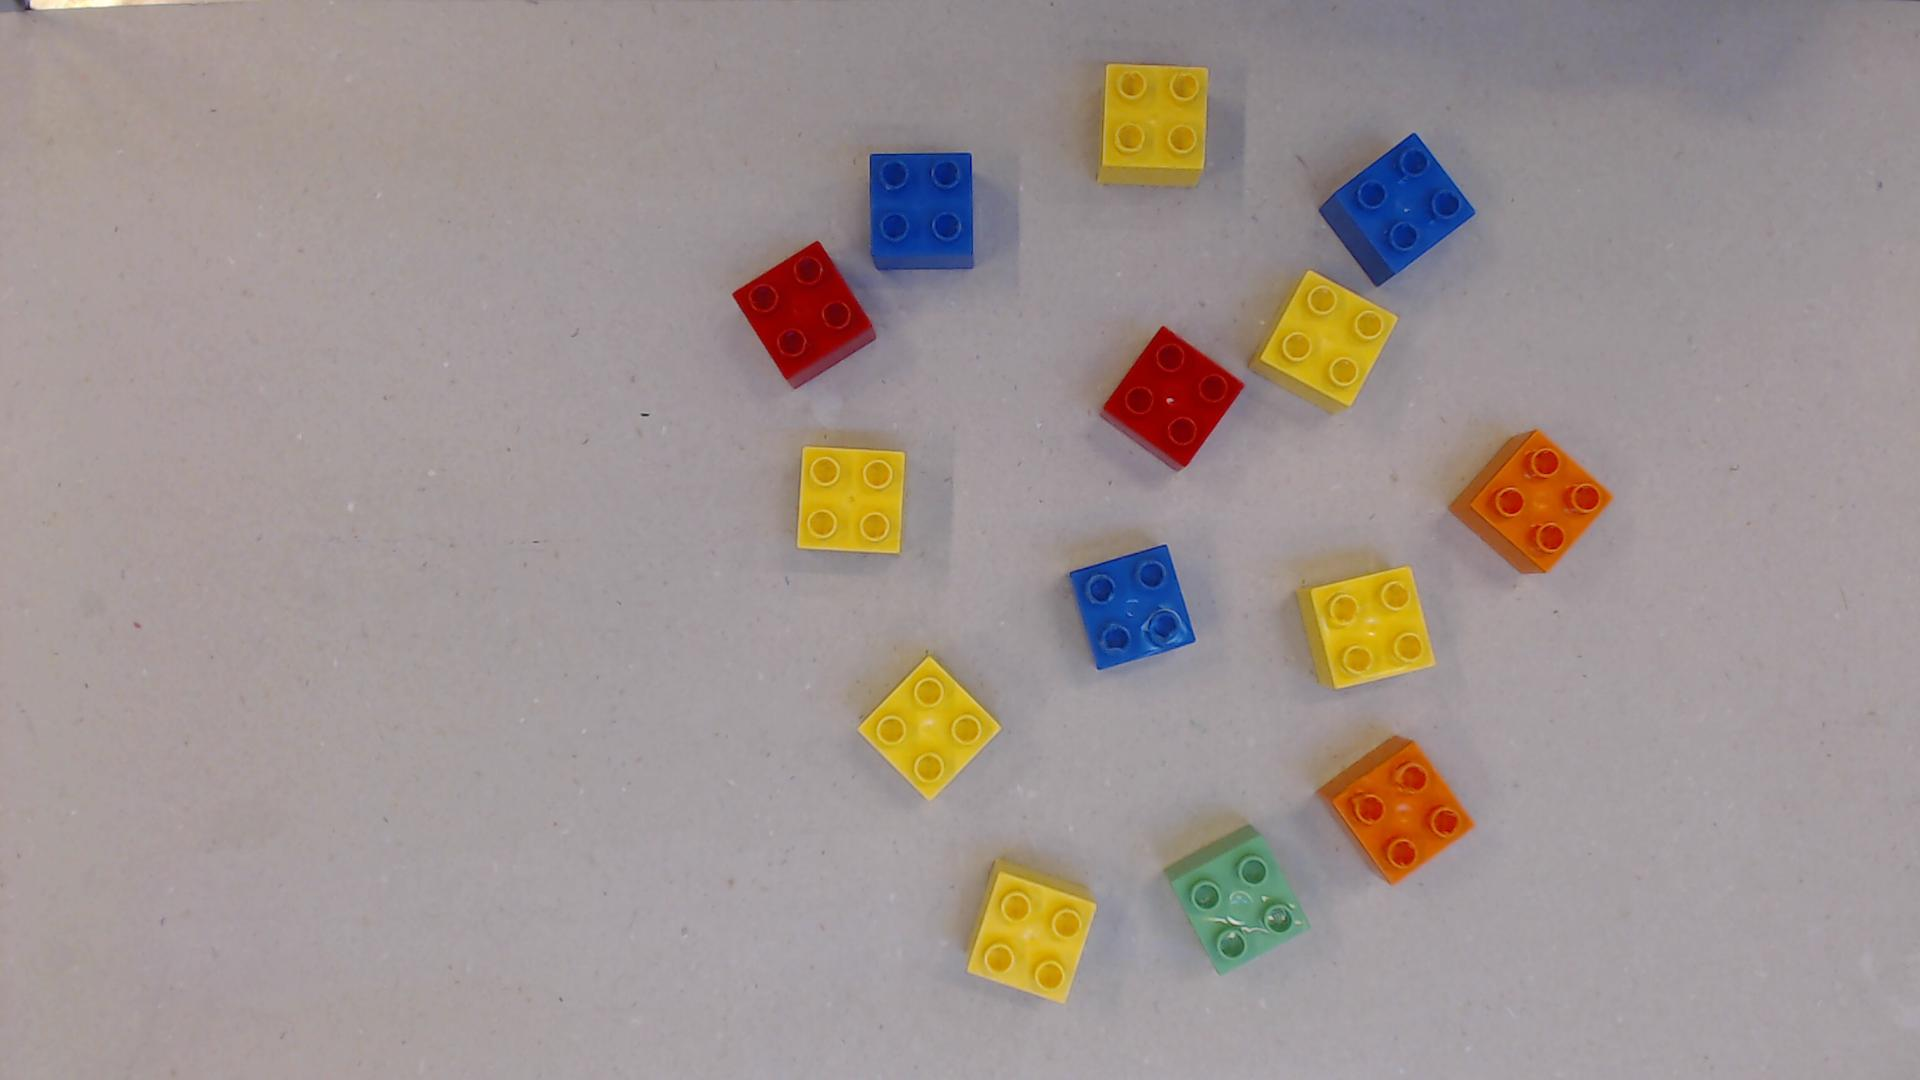
\includegraphics[width=0.69\textwidth]{figures/orig_pic.jpg}
	\caption{Original picture taken by the webcam attached to the robot.}
	\label{fig:orig_pic}
\end{figure}

\section{Format Conversion}
The original picture taken by the webcam is in RGB and is converted to a chromaticity image. This is done using \autoref{eq:rgb_to_rgi}:

\begin{equation}\label{eq:rgb_to_rgi}
	r=\frac{R}{R+G+B}, ~g=\frac{G}{R+G+B}, ~I=\frac{R+G+B}{3}
\end{equation}

Chromaticity is given from the chromaticity plane. This is shown in \autoref{fig:chrom_plane}. This is done since the colours are being normalised to avoid influence by illumination. Then the colour description is supplemented by an intensity as calculated in \autoref{eq:rgb_to_rgi}. This will be referred to as RGI and the conversion is RGB to RGI.


\begin{figure}[H]
	\centering
	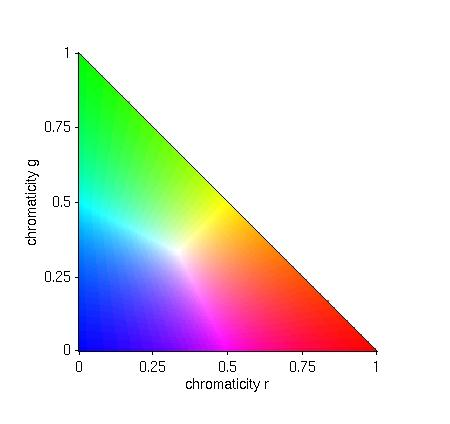
\includegraphics[width=0.7\textwidth]{figures/chrom_plane}
	\caption{Chromaticity plane}
	\label{fig:chrom_plane}
\end{figure}

The advantage of this is, that this should allow for colour thresholding on any image as it disregards illumination.

\section{Background Subtraction}
The background of the image is subtracted to ease the localisation of the brick edges. This is done by taking a picture of the surface without any bricks as a background image from the exact same position as the original image.
To avoid unwillingly removing any objects from the new image generated a threshold is set fro specific pixel values.

Firstly the RGB image of the background is converted to an RGI image. The subtraction is then performed pixel-wise using the formula shown in \autoref{eq:back_sub}. The subtraction is done using the two RGI images.

\begin{equation}\label{eq:back_sub}
	F(x,y) = I(x,y) - B(x,y)
\end{equation}

The thresholding is done by setting a threshold a value and doing a pixel-wise comparison. Should any of the channels have a higher value than the threshold, the pixel will be kept as a non-background pixel value.

\section{Colour Thresholding}
The colour thresholding is done to separate the individual brick colours from each other. The thresholding is done by comparing the pixel values of the RGI image to a set threshold for each channel. Firstly a threshold is applied to the intensity channel. This is done to rule out coloured pixels which may be indistinguishable because of too small an intensity. 

The colour thresholding is then made on the image. This is done for every brick colour used in the project by setting thresholds for both $r$ and $g$ channels to match the desired colour of a brick. A small pseudocode example is shown below:
\lstset{language=Pascal}
\begin{lstlisting}[frame=single]
if: 
	TH_r_min < r < TH_r_max AND
	TH_g_min < g < TH_g_max
then: object pixel
else: non-object pixel
\end{lstlisting}

If the pixel satisfies the set thresholds for the two channels, it is marked as a binary $1$ in an output image.

To set the thresholds fro the different colours in the $r$ and $g$ channels the RGI image is analysed. By cropping the picture to match each brick colour and analysing each for the chosen colour the thresholds are found by taking the $5\%$ and $95\%$ percentiles are found and used as the thresholds for each colour.

\section{Noise Removal}
The noise removal also known as morphology is done as the images generated from thresholding can contain some outliers which is not entire bricks but is recognised inside the threshold limits. Furthermore the bricks recognised contain some holes which is preferred to be filled.

To do this morphology the \textit{hit} and \textit{fit} operations are taken in use also known as dilation and erosion. These are firstly used to close the holes in the bricks and then opening to remove noise.
For this kernels for both dilation and erosion are defined. The functionality of both dilation and erosion is shown in \autoref{fig:dil_eros}

\begin{figure}
	\centering
	\begin{subfigure}[b]{0.45\textwidth}
		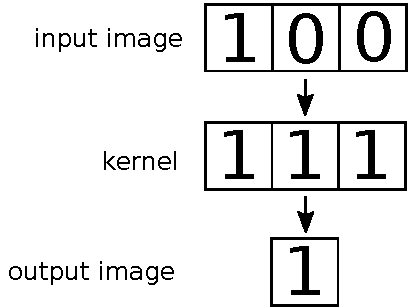
\includegraphics[width=\textwidth]{figures/dilation}
		\caption{Dilation kernel}
		\label{fig:dilation}
	\end{subfigure}
	\begin{subfigure}[b]{0.45\textwidth}
		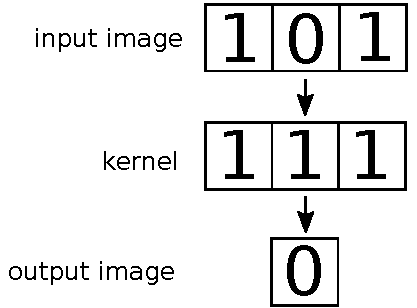
\includegraphics[width=\textwidth]{figures/erosion}
		\caption{Erosion kernel}
		\label{fig:erosion}
	\end{subfigure}
	\caption{Example of dilation and erosion kernel.}
	\label{fig:dil_eros}
\end{figure}

\section{BLOB Analysis}
The BLOB analysis is made to find the location of the bricks but also to find the rotation of the bricks to pick them up correctly. To do this a classification is necessary. This is done using the Grassfire algorithm with 4-connectivity. This enumerates each pixel belonging to a BLOB on the images for each of the brick colours.

The next step is finding the centre of the BLOBs or bricks, done by using centre of mass. This is calculated using the formulas shown in \autoref{eq:mass_centre}.

\begin{equation}\label{eq:mass_centre}
	x_m = \frac{1}{N}\sum_{i \in object}x_i, ~y_m= \frac{1}{N}\sum_{i \in object}y_i 
\end{equation}


To be able to pick up the bricks properly, the rotation of the bricks must be found. By calculating the distance from each pixel, forming a BLOB of a brick, to the centre of the BLOB the four corners are found by finding the four pixels furthest away from the centre. By defining four vectors from the centre of the brick to each corner the angles are calculated and by that the rotation. This is found by finding the mean of the four angles. In illustration of the vectors defined of the BLOB is shown in \autoref{fig:rot_fig}.

\begin{figure}[H]
	\centering
	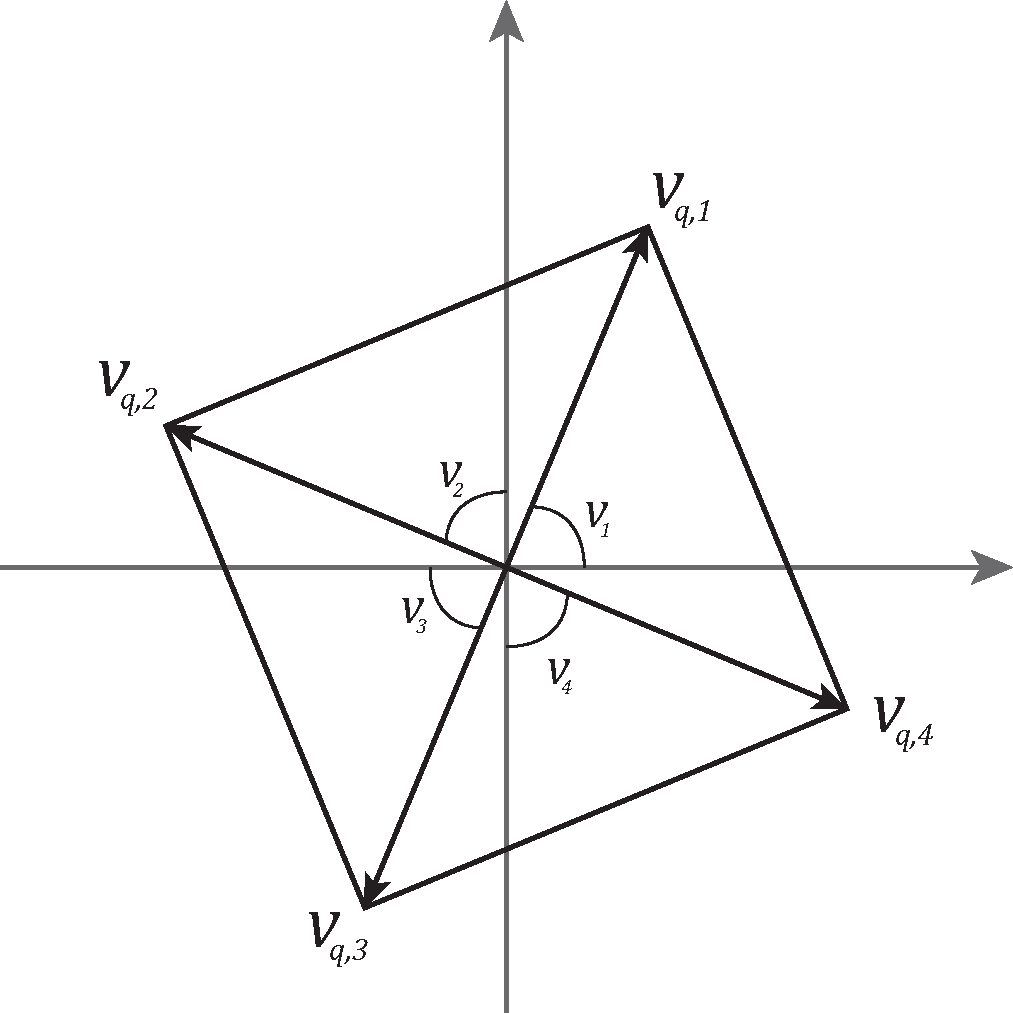
\includegraphics[width=0.65\textwidth]{figures/rot_fig}
	\caption{Rotations found from vectors and corners in a BLOB}
	\label{fig:rot_fig}
\end{figure}

The final result of the computer vision part yields five arrays with brick information of each colour and brick. This includes position and rotation used to locate and pick up the bricks. A final informational image of this including a directional vector showing the rotation is shown in \autoref{fig:fin_pic}.

\begin{figure}[H]
	\centering
	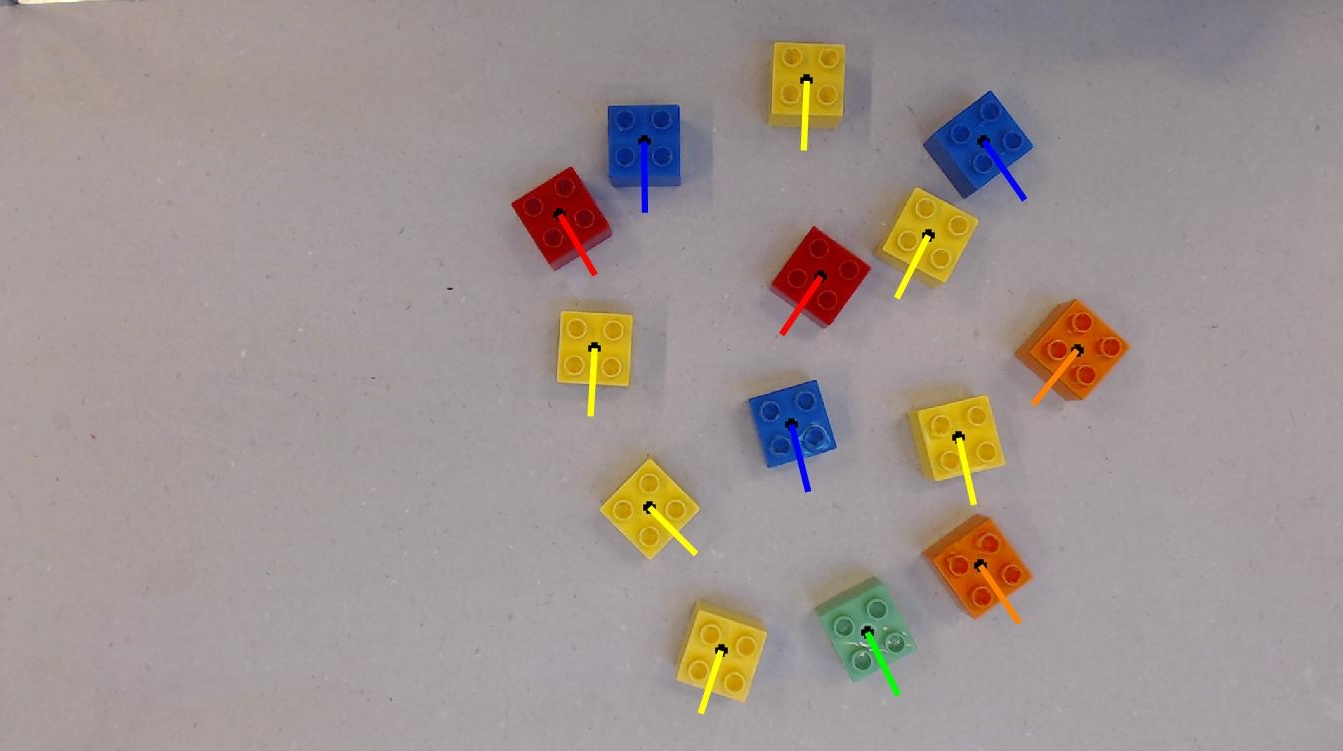
\includegraphics[width=\textwidth]{figures/fin_pic.jpg}
	\caption{Final informational image including brick centre and rotation directional vector.}
	\label{fig:fin_pic}
\end{figure}